\documentclass[11pt]{article}

\usepackage[margin=1in]{geometry}
\usepackage{graphicx}
\usepackage{booktabs}
\usepackage{siunitx}
\usepackage{xcolor}
\usepackage{hyperref}
\usepackage{caption}
\usepackage{amsmath}
\usepackage{multirow}
\usepackage{fancyhdr}

\hypersetup{colorlinks=true, linkcolor=blue!50!black, citecolor=blue!50!black, urlcolor=blue!50!black}

\title{\textbf{In-Order Superscalar Issue-Width Analysis} \\[4pt]
\large RSVP RISC-V Emulator (32I) --- NPU-Accelerated $256\times256$ Matrix Multiply}
\author{RSVP Project}
\date{\today}

\pagestyle{fancy}
\fancyhf{}
\fancyhead[L]{Superscalar Issue-Width Analysis}
\fancyhead[R]{\thepage}
\renewcommand{\headrulewidth}{0.3pt}

\begin{document}
\maketitle

\begin{abstract}
\noindent
RSVP's \texttt{32I} tree implements an additive, in-order superscalar issue
mode alongside its scalar five-stage pipeline: an $n$-wide fetch window per
cycle, in-order dispatch and writeback, no speculation, no register renaming.
This report measures how that mode performs across compiler optimization
level ($\texttt{-O0}$ to $\texttt{-O3}$) and issue width ($n=1$ to $10$) on
the workload the model was developed and validated against --- a
$256\times256$ tiled matrix multiply run on RSVP's memory-mapped NPU
accelerator (template~2, custom-0 tile-transfer instructions). All data here
was produced by \texttt{32I/tests/npu/analyze\_superscalar.py}, a harness
that compiles the workload once per optimization level and traces it in
scalar mode and in superscalar mode at every issue width against the
\emph{same} binary, so cycle counts are directly comparable within a level.
\end{abstract}

\tableofcontents

% ---------------------------------------------------------------------
\section{Background}
% ---------------------------------------------------------------------

The superscalar mode (documented in \texttt{docs/superscalar.md} and its
companion progress log \texttt{docs/superscalar-progress.md}) is a classic
first-generation design: \texttt{fetch\_n()} reads $n$ consecutive words,
\texttt{decode\_all()} decodes them, \texttt{hazard\_scan()} picks the
largest hazard-free prefix $m \le n$ of that window, and
\texttt{execute\_m()}/\texttt{read\_m()}/\texttt{writeback\_m()} process that
prefix in program order before \texttt{pc} advances by $4m$. The window
closes at:
\begin{itemize}
  \item \textbf{a control hazard} --- a branch, \texttt{jal}, or
    \texttt{jalr} always ends the window right after itself (no
    speculation is implemented);
  \item \textbf{a RAW hazard} --- an instruction that reads a register an
    earlier slot in the same window writes;
  \item \textbf{a structural (memory-port) hazard} --- two instructions
    that contend for the same memory-port class (\texttt{NONE} /
    \texttt{BANK\_A} / \texttt{BANK\_B} / \texttt{STORE}), modeling a small,
    plausible set of physical read/write ports rather than one shared bus.
\end{itemize}
WAW and WAR are structurally impossible to violate in this model rather than
being actively scanned for: writeback commits slots in window order, and
every slot's register read happens before any slot's write lands, so both
hazard classes resolve for free. None of these rules are required for
\emph{correctness} --- \texttt{execute\_m()}/\texttt{read\_m()}/
\texttt{writeback\_m()} process every slot sequentially regardless, so even a
genuinely aliasing pair placed in the same window would still produce the
right result. They exist purely to model plausible hardware resource limits,
and the memory-hazard rule specifically went through three iterations before
settling on ``two instructions conflict only if they share the exact same
memory-port class'' (see \texttt{docs/superscalar-progress.md}, \S3, for the
full history).

The workload under test is the $256\times256$ NPU-accelerated tiled matrix
multiply (\texttt{matmul\_256\_t2.c}, template~2): each $16\times16$ tile is
loaded with the custom-0 \texttt{load\_a}/\texttt{load\_b} instructions
(contiguous 256-word block transfers into separate NPU SRAM banks), the
matrix-multiply-accumulate is triggered with a store to the NPU's MAC
register, and the result tile is written back with a strided store. This is
the workload the superscalar model was actually developed and correctness-
verified against (bit-exact final register state vs.\ the scalar pipeline,
at every issue width tested, across both NPU templates, multiple sizes, and
every stage of the hazard-model's evolution).

% ---------------------------------------------------------------------
\section{Methodology}
% ---------------------------------------------------------------------

For each optimization level $\texttt{-O0} \ldots \texttt{-O3}$:
\begin{enumerate}
  \item the workload is cross-compiled once for \texttt{rv32im}
    (\texttt{riscv64-unknown-elf-gcc}, bare-metal, via
    \texttt{tests/python/start.s}/\texttt{link.ld});
  \item the resulting binary is traced once in scalar mode, and once in
    superscalar mode at each issue width $n=1,\dots,10$ ---
    \emph{the same binary every time}, so only the issue mechanism varies
    within a level, not the code;
  \item cycles, total retired instructions, and the per-cycle
    co-issue-count histogram are parsed from each trace.
\end{enumerate}
All 44 runs (4 levels $\times$ [scalar + $n{=}1..10$]) halted normally (the
program's own \texttt{j \_end} loop, this codebase's halt idiom), and total
retired-instruction count was confirmed invariant across issue width for a
fixed level in every case --- issue width changes \emph{when} instructions
retire, never \emph{how many} retire. The full 4-level $\times$ 11-run raw
sweep (cycles, instructions, and co-issue histograms) is archived alongside
this report as \texttt{data/superscalar\_sweep\_n10.json}.

% ---------------------------------------------------------------------
\section{Results}
% ---------------------------------------------------------------------

\subsection{Cycles vs.\ optimization level}

Figure~\ref{fig:cycles-vs-opt} shows the scalar-pipeline ($n=1$) cycle count
at each optimization level. \texttt{-O0}'s $279{,}303$ cycles dwarf every
optimized level by roughly an order of magnitude; \texttt{-O1}
($26{,}525$), \texttt{-O2} ($26{,}763$), and \texttt{-O3} ($21{,}552$) are
within a narrow band of each other, with \texttt{-O3} the clear low point.
Notably, \texttt{-O1} and \texttt{-O2} are within $1\%$ of one another on
this workload --- \texttt{-O2}'s usual advantage over \texttt{-O1} doesn't
show up here, most likely because the hand-tiled NPU loop is already tight
enough that \texttt{-O2}'s extra optimizations (vectorization, more
aggressive inlining) have little left to exploit on top of what \texttt{-O1}
already does.

\begin{figure}[htbp]
  \centering
  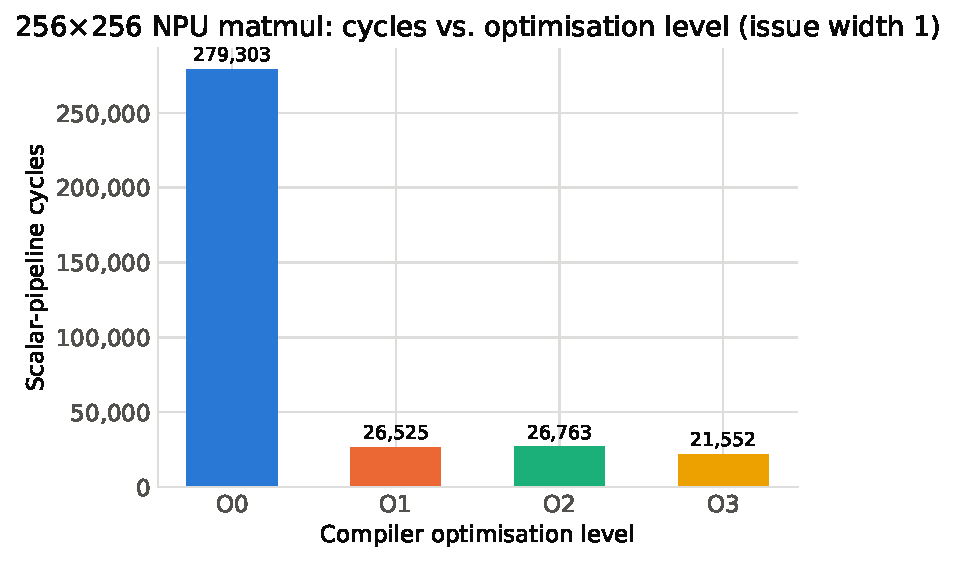
\includegraphics[width=0.72\textwidth]{figures/fig1_cycles_vs_optimisation.pdf}
  \caption{Scalar-pipeline (issue width 1) cycle count by optimization
  level, $256\times256$ NPU matmul.}
  \label{fig:cycles-vs-opt}
\end{figure}

\subsection{Cycles vs.\ issue width}

Figure~\ref{fig:cycles-vs-n} plots cycle count against issue width for all
four optimization levels on one log-scaled axis (a linear axis would
compress \texttt{-O1}--\texttt{-O3} into a single line against
\texttt{-O0}'s much larger scale). Every curve is monotonically
non-increasing and flattens out well before $n=10$: \texttt{-O0} converges
at $n=5$, \texttt{-O1} at $n=4$, and \texttt{-O2}/\texttt{-O3} at $n=6$ ---
after which widening the window further buys, at most, one or two cycles
out of several thousand (a sub-$0.1\%$ tail). The full per-level, per-$n$
numbers are in Table~\ref{tab:full-sweep}.

\begin{figure}[htbp]
  \centering
  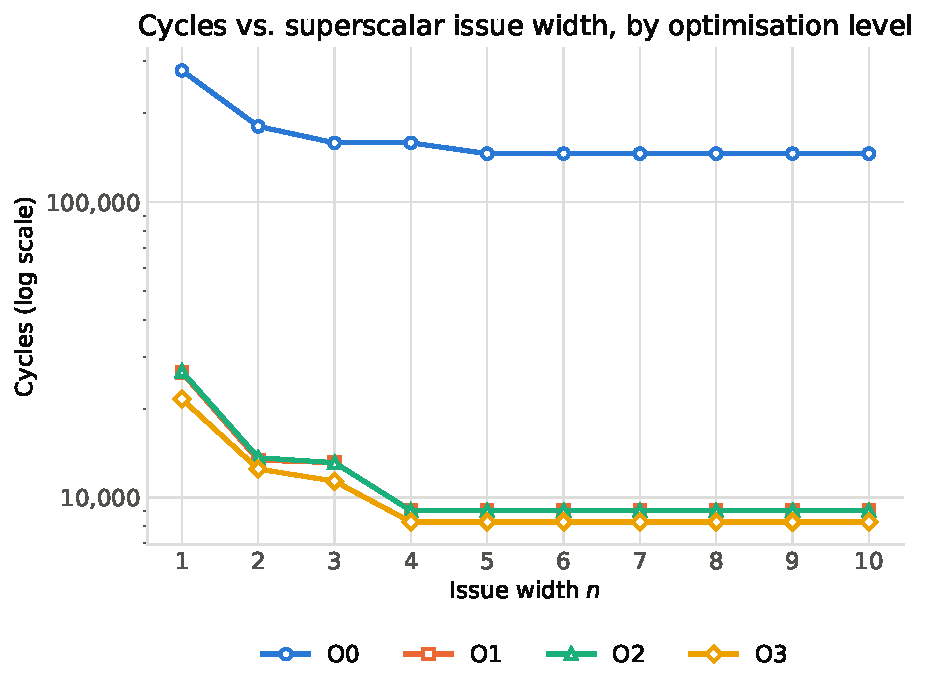
\includegraphics[width=0.8\textwidth]{figures/fig2_cycles_vs_issue_width.pdf}
  \caption{Cycles vs.\ superscalar issue width $n$, all four optimization
  levels on one log-scaled axis.}
  \label{fig:cycles-vs-n}
\end{figure}

\subsection{IPC vs.\ issue width}

Figure~\ref{fig:ipc-vs-n} shows average IPC (retired instructions divided by
cycles) against issue width. \texttt{-O1} and \texttt{-O2} track each other
almost exactly and top out just under $2.97$ IPC; \texttt{-O3} converges to
a lower $2.61$ IPC despite having the fewest total cycles of any level, and
\texttt{-O0} converges lowest of all at $1.91$ IPC despite having by far the
most instruction-level redundancy available to exploit. This is the
report's central finding, expanded on in \S\ref{sec:discussion}: raw
instruction-level parallelism (which \texttt{-O0} has the most of) and
\emph{realized} IPC under this hazard model are not the same thing.

\begin{figure}[htbp]
  \centering
  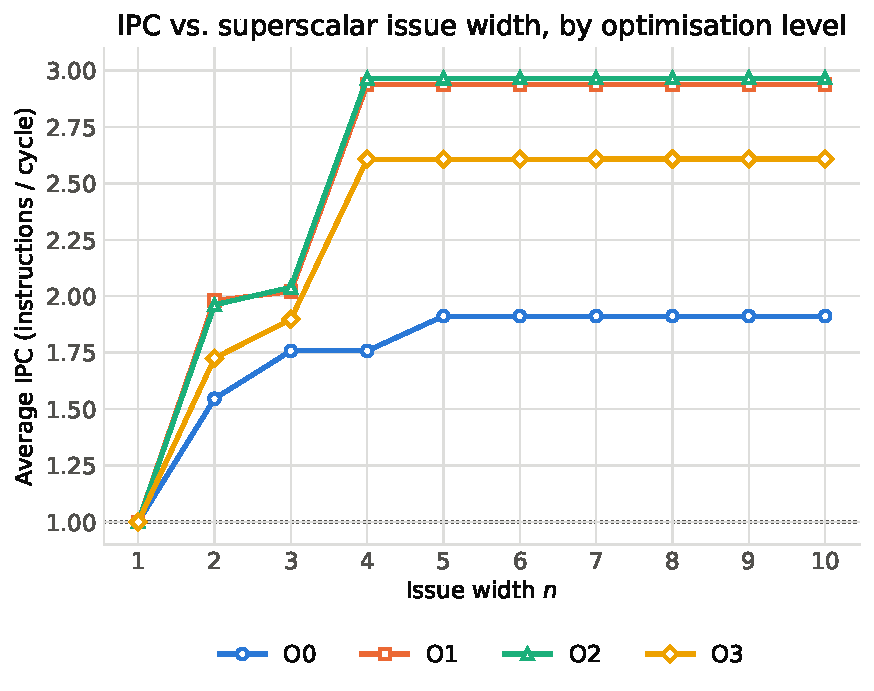
\includegraphics[width=0.8\textwidth]{figures/fig3_ipc_vs_issue_width.pdf}
  \caption{Average IPC vs.\ superscalar issue width $n$, all four
  optimization levels on one axis.}
  \label{fig:ipc-vs-n}
\end{figure}

\subsection{Speedup vs.\ issue width}

Figure~\ref{fig:speedup-vs-n} restates the same cycle data as speedup
relative to each level's own scalar baseline. The shape is consistent
across all four levels: roughly $70$--$80\%$ of the achievable speedup
lands at $n=2$ already, and every level is within a percent or two of its
final asymptote by $n=4$.

\begin{figure}[htbp]
  \centering
  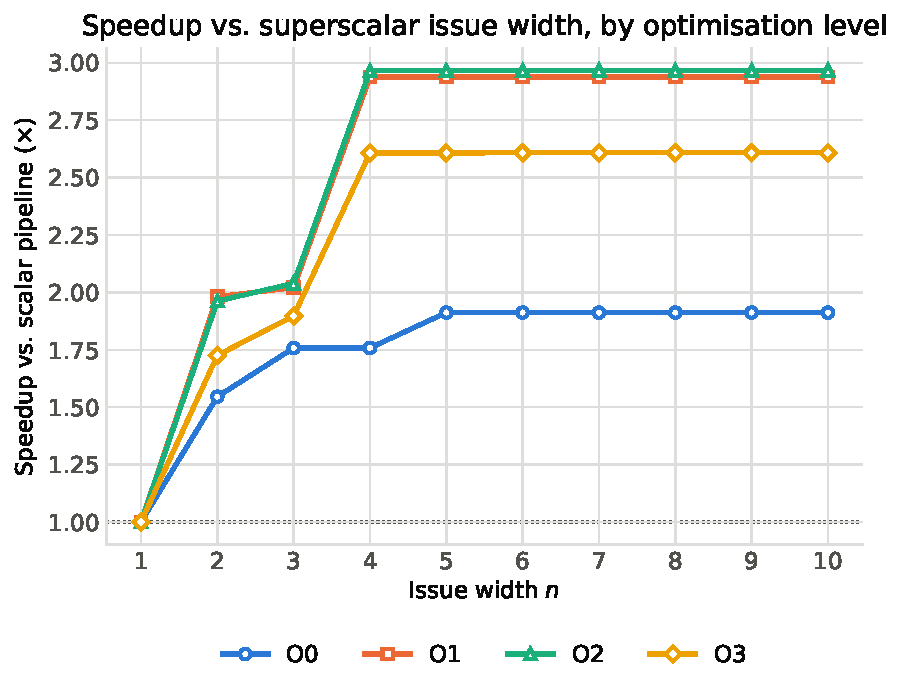
\includegraphics[width=0.8\textwidth]{figures/fig4_speedup_vs_issue_width.pdf}
  \caption{Speedup vs.\ scalar pipeline, by issue width $n$ and optimization
  level.}
  \label{fig:speedup-vs-n}
\end{figure}

\subsection{Best achievable speedup by level}

Figure~\ref{fig:best-speedup} summarizes the best speedup each level
reaches within $n \le 10$. \texttt{-O2} is the overall winner at
$2.966\times$, narrowly ahead of \texttt{-O1} at $2.938\times$;
\texttt{-O3}'s already-tight scheduling leaves the least slack for co-issue
and comes in lowest of the optimized levels at $2.608\times$;
\texttt{-O0}'s raw redundancy is real but caps out well below the optimized
levels at $1.912\times$.

\begin{figure}[htbp]
  \centering
  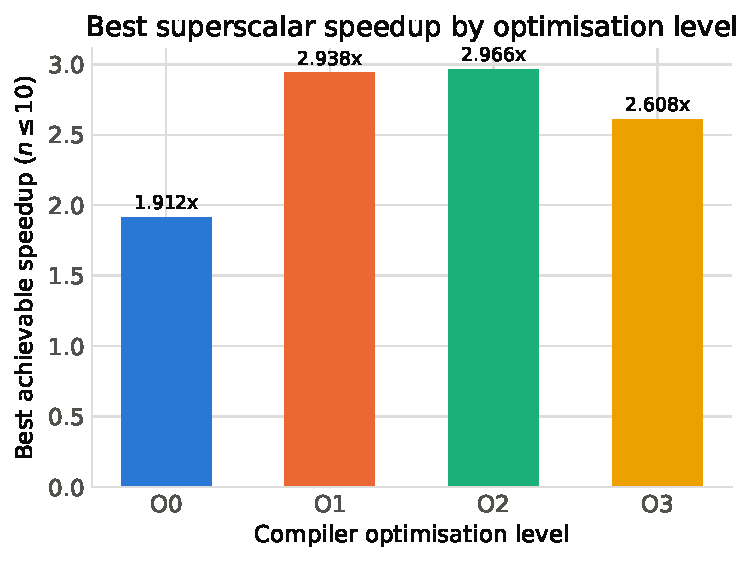
\includegraphics[width=0.72\textwidth]{figures/fig5_best_speedup_by_level.pdf}
  \caption{Best speedup achieved within $n \le 10$, by optimization level.}
  \label{fig:best-speedup}
\end{figure}

\subsection{Co-issue width distribution}

Figure~\ref{fig:coissue} shows what fraction of cycles issue $1, 2, \dots$
instructions together, at each level's converged issue width. \texttt{-O0}
and \texttt{-O3} show a smoother spread across co-issue widths, while
\texttt{-O1} and \texttt{-O2} are dominated by a bimodal
1-instruction/4-instruction split with a long, thin tail in between ---
consistent with a K-loop body of a handful of independent
address/load/store/MAC instructions followed by a lone branch every
iteration (see \S\ref{sec:discussion}).

\begin{figure}[htbp]
  \centering
  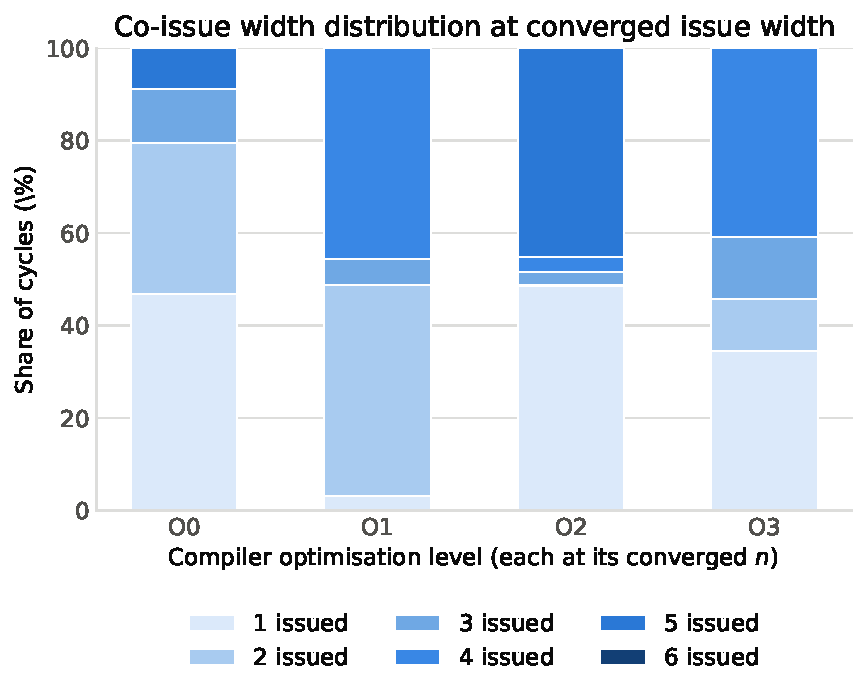
\includegraphics[width=0.76\textwidth]{figures/fig6_coissue_distribution.pdf}
  \caption{Distribution of instructions co-issued per cycle at each level's
  converged issue width ($n=5,4,6,6$ for O0--O3 respectively).}
  \label{fig:coissue}
\end{figure}

\clearpage
\subsection{Full numerical sweep}

Table~\ref{tab:full-sweep} lists every measured point: cycles, average IPC,
and speedup vs.\ scalar, for all four optimization levels at issue widths
$1$ through $10$.

\begin{table}[htbp]
\centering
\caption{Full $256\times256$ NPU matmul sweep: cycles, average IPC, and
speedup vs.\ the scalar baseline, by optimization level and issue width.}
\label{tab:full-sweep}
\begin{tabular}{cr rrr}
\toprule
Level & $n$ & Cycles & Avg.\ IPC & Speedup \\
\midrule
\multirow{10}{*}{\texttt{-O0}\ (279{,}303 instr.)}
 & 1  & 279{,}303 & 1.0000 & 1.000$\times$ \\
 & 2  & 180{,}664 & 1.5460 & 1.546$\times$ \\
 & 3  & 158{,}877 & 1.7580 & 1.758$\times$ \\
 & 4  & 158{,}876 & 1.7580 & 1.758$\times$ \\
 & 5  & 146{,}072 & 1.9121 & 1.912$\times$ \\
 & 6  & 146{,}072 & 1.9121 & 1.912$\times$ \\
 & 7  & 146{,}072 & 1.9121 & 1.912$\times$ \\
 & 8  & 146{,}072 & 1.9121 & 1.912$\times$ \\
 & 9  & 146{,}072 & 1.9121 & 1.912$\times$ \\
 & 10 & 146{,}072 & 1.9121 & 1.912$\times$ \\
\midrule
\multirow{10}{*}{\texttt{-O1}\ (26{,}525 instr.)}
 & 1  & 26{,}525 & 1.0000 & 1.000$\times$ \\
 & 2  & 13{,}388 & 1.9813 & 1.981$\times$ \\
 & 3  & 13{,}128 & 2.0205 & 2.020$\times$ \\
 & 4  & 9{,}028  & 2.9381 & 2.938$\times$ \\
 & 5  & 9{,}028  & 2.9381 & 2.938$\times$ \\
 & 6  & 9{,}028  & 2.9381 & 2.938$\times$ \\
 & 7  & 9{,}027  & 2.9384 & 2.938$\times$ \\
 & 8  & 9{,}027  & 2.9384 & 2.938$\times$ \\
 & 9  & 9{,}027  & 2.9384 & 2.938$\times$ \\
 & 10 & 9{,}027  & 2.9384 & 2.938$\times$ \\
\midrule
\multirow{10}{*}{\texttt{-O2}\ (26{,}763 instr.)}
 & 1  & 26{,}763 & 1.0000 & 1.000$\times$ \\
 & 2  & 13{,}641 & 1.9620 & 1.962$\times$ \\
 & 3  & 13{,}123 & 2.0394 & 2.039$\times$ \\
 & 4  & 9{,}026  & 2.9651 & 2.965$\times$ \\
 & 5  & 9{,}025  & 2.9654 & 2.965$\times$ \\
 & 6  & 9{,}023  & 2.9661 & 2.966$\times$ \\
 & 7  & 9{,}023  & 2.9661 & 2.966$\times$ \\
 & 8  & 9{,}022  & 2.9664 & 2.966$\times$ \\
 & 9  & 9{,}022  & 2.9664 & 2.966$\times$ \\
 & 10 & 9{,}022  & 2.9664 & 2.966$\times$ \\
\midrule
\multirow{10}{*}{\texttt{-O3}\ (21{,}552 instr.)}
 & 1  & 21{,}552 & 1.0000 & 1.000$\times$ \\
 & 2  & 12{,}488 & 1.7258 & 1.726$\times$ \\
 & 3  & 11{,}358 & 1.8975 & 1.898$\times$ \\
 & 4  & 8{,}267  & 2.6070 & 2.607$\times$ \\
 & 5  & 8{,}266  & 2.6073 & 2.607$\times$ \\
 & 6  & 8{,}265  & 2.6076 & 2.608$\times$ \\
 & 7  & 8{,}265  & 2.6076 & 2.608$\times$ \\
 & 8  & 8{,}264  & 2.6079 & 2.608$\times$ \\
 & 9  & 8{,}264  & 2.6079 & 2.608$\times$ \\
 & 10 & 8{,}264  & 2.6079 & 2.608$\times$ \\
\bottomrule
\end{tabular}
\end{table}

\clearpage
% ---------------------------------------------------------------------
\section{Discussion}
\label{sec:discussion}
% ---------------------------------------------------------------------

\paragraph{Instruction count is invariant; only scheduling changes.}
For a fixed optimization level, total retired instructions are identical at
every issue width (confirmed exactly for all 44 runs) --- the superscalar
mode is purely a scheduling change on top of a fixed instruction stream, not
a different program. This makes the cycle-count reduction in
Figure~\ref{fig:cycles-vs-n} attributable entirely to co-issue, with nothing
else confounding the comparison.

\paragraph{Almost all the achievable speedup lands by $n=2$--$4$.} Every
level's curve is sharply concave: the first doubling of issue width
captures the large majority of the eventual speedup, and every level has
converged (bit-for-bit identical cycle count) by $n=6$ at the latest.
Widening the model's issue window from 6 to 10 --- a $67\%$ increase in
hardware width --- changes total cycles by at most a few units out of
several thousand at any level. For this workload, a 4--6-wide issue window
already captures essentially all of the benefit a wider one would provide.

\paragraph{Optimized code parallelizes \emph{better}, not just \emph{starts
lower}.} A natural guess would be that \texttt{-O0}'s extra redundant
instructions (spills, address recomputation, etc.) are ``free'' parallelism
that optimization removes, so optimized code should have \emph{less} room
to benefit from wider issue. The IPC data says the opposite:
\texttt{-O1}/\texttt{-O2} reach nearly $3.0$ average IPC, while \texttt{-O0}
tops out at $1.91$. The redundant instructions \texttt{-O0} carries are not
uniformly parallel with their neighbors --- many are on the dependency chain
they exist to serve (e.g.\ a spilled value reloaded immediately before the
instruction that consumes it), so they extend RAW chains rather than
filling co-issue slots. Optimized code's tighter dependency structure
turns out to co-issue more effectively under this in-order, no-forwarding
model, not less.

\paragraph{The register-argument bottleneck, not the branch, is the real
floor.} Tracing showed the K-loop body's steady-state co-issue pattern is a
5-wide group (\texttt{load\_a} + \texttt{load\_b} + \texttt{sw} (MAC
trigger) + two address-increment \texttt{add}s) followed by the loop-closing
\texttt{bne} executing alone. The intuitive explanation is that the branch
is the bottleneck; loop-unrolling experiments (recorded in
\texttt{docs/superscalar-progress.md}, \S8) tested this directly and found
otherwise. Removing the branch by fully unrolling the K-loop saved far less
than predicted ($678$ of a projected $\sim\!4096$ cycles at \texttt{-O2},
$n{=}6$), because the compiler's fully-unrolled code replaced the branch
with a \texttt{lui}+\texttt{add} address-rebuild pair that has the exact
same ``alone in a wide window'' shape --- a RAW hazard where \texttt{add}
consumes the register \texttt{lui} just wrote. The real constraint is
structural: \texttt{load\_a}/\texttt{load\_b}/\texttt{store\_c} each take a
register argument, and \emph{something} must compute that argument's value
in the cycle immediately before it, and that producer can never co-issue
with the consumer under this no-forwarding model. Both the branch and the
address computation are instances of the same underlying limit, not two
independent bottlenecks --- which is why removing one just exposes the
other at close to the same cost.

\paragraph{\texttt{-O2} wins, but not by a wide margin over \texttt{-O1}.}
\texttt{-O2}'s $2.966\times$ best speedup edges out \texttt{-O1}'s
$2.938\times$ by under $1\%$, and their IPC and cycle-count curves in
Figures~\ref{fig:cycles-vs-n}--\ref{fig:ipc-vs-n} are visually
indistinguishable. \texttt{-O3}, despite having the fewest total
instructions and fewest absolute cycles of any level, has the
\emph{weakest} co-issue behavior of the three optimized levels ---
consistent with the general pattern that more aggressive scheduling at
\texttt{-O3} leaves less independent, easily-co-issuable structure behind.

\paragraph{Threats to validity / scope.} All numbers in this report are for
one workload (a $256\times256$ NPU-accelerated tiled matmul) compiled with
one toolchain, run at one random seed. The superscalar model itself has no
speculation and no register renaming, so these results characterize a
specific, conservative point in the design space --- a design with
predict-taken branch speculation or forwarding (both discussed as open
future work in \texttt{docs/superscalar-progress.md}, \S9) would likely
change both the absolute numbers and which optimization level wins.

% ---------------------------------------------------------------------
\section{Conclusion}
% ---------------------------------------------------------------------

Across every optimization level tested, this in-order superscalar model
converges to a stable speedup well within an issue width of $6$, with the
large majority of the benefit already realized by $n=2$--$4$. \texttt{-O2}
achieves the best overall speedup ($2.966\times$ at $n \ge 6$), narrowly
ahead of \texttt{-O1} ($2.938\times$); \texttt{-O3}'s tighter scheduling
leaves comparatively less co-issue opportunity ($2.608\times$); and
\texttt{-O0}, despite the most redundant instructions, converges lowest of
all ($1.912\times$) because that redundancy mostly extends dependency
chains rather than supplying independent work. Under the current
no-forwarding, no-speculation hazard model, the practical ceiling on this
workload is set less by any single hazard type than by a recurring
structural pattern: an address or branch-condition value computed one
instruction before it is consumed, which can never co-issue with its
consumer regardless of window width. Moving past that floor is identified
as future work requiring either register forwarding or branch speculation,
not a wider issue window.

\vspace{1em}
\noindent\textit{Reproducing this report:} \texttt{python3
32I/tests/npu/analyze\_superscalar.py --max-n 10 --json
data/superscalar\_sweep\_n10.json}, run from
\texttt{32I/tests/npu/}, with \texttt{--src} pointed at the desired matmul
source. Figures were generated from that JSON by
\texttt{make\_plots.py} (archived alongside this report).

\end{document}
